\include{template}
\cfoot{}

\begin{document}

\begin{header}
Rappels de collège
\end{header}

\noindent
\emph{Entourer les bonnes réponses. Il peut y avoir plusieurs bonnes réponses.}

\begin{enumerate}

\item Un corps pur est une substance :
\begin{multicols}{2}
\begin{enumerate}
\item que l'on trouve souvent dans la nature
\item qui ne pollue pas
\item constituée de particules identiques
\item constituée de particules différentes
\end{enumerate}
\end{multicols}

\item On mélange de l'eau et de l'huile.
\begin{multicols}{2}
\begin{enumerate}
\item Les deux liquides se distinguent à l'œil nu
\item On obtient un mélange homogène
\item On obtient un mélange hétérogène
\item On obtient un corps pur
\item Les deux liquides sont miscibles
\item Les deux liquides sont non miscibles
\end{enumerate}
\end{multicols}

\item L'air est :
\begin{multicols}{2}
\begin{enumerate}
\item un corps pur
\item un mélange homogène de plusieurs gaz
\item un mélange hétérogène de plusieurs gaz
\item composé majoritairement $\diazote$
\item composé majoritairement de $\dioxygene$
\end{enumerate}
\end{multicols}

\item Pour de l'eau pure, le passage de l'état solide à l'état liquide :
\begin{multicols}{2}
\begin{enumerate}
\item s'appelle la fusion
\item s'appelle la solidification
\item se fait à une température de $\unit{100}{\celsius}$
\item se fait à une température de $\unit{0}{\celsius}$
\end{enumerate}
\end{multicols}


\item La masse volumique $\rho$ (\emph{rhô}) d'un corps de masse $m$ et de volume $V$ est donnée par :
\begin{multicols}{3}
\begin{enumerate}
\item $\rho= \dfrac{m}{V}$
\item $\rho= m \times V$
\item $\rho= \dfrac{V}{m}$
\end{enumerate}
\end{multicols}

\item Jusqu'en novembre 2018, le kilogramme était défini par rapport à un étalon réalisé dans un alliage de platine de masse volumique $\unit{21\,186}{\kilo\gram/\meter^3}$.
Par définition, ce cylindre a une masse de $\unit{1}{\kilo\gram}$.
Son volume est d'environ :
\begin{multicols}{3}
\begin{enumerate}
\item $\unit{47}{m^3}$
\item $\unit{47}{cm^3}$
\item $\unit{47}{\liter}$
\item $\unit{47}{\milli\liter}$
\item $\unit{0{,}047}{\liter}$
\item $\unit{0{,}047}{\deci\meter^3}$
\end{enumerate}
\end{multicols}

\begin{figure}[b]
\center
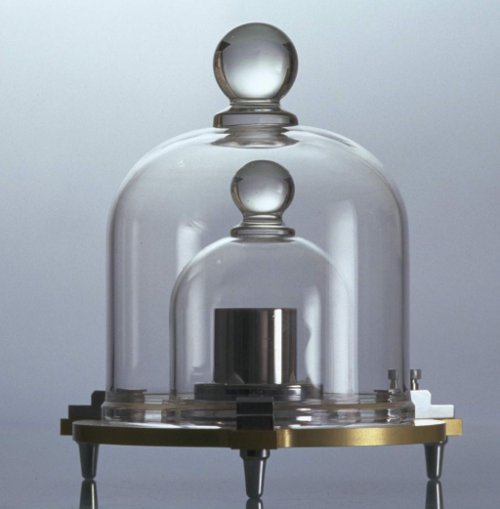
\includegraphics[scale=0.19]{images/kilogramme_etalon.jpg}
\caption{\emph{LE} kilogramme étalon conservé sous très haute surveillance près de Paris.}
\end{figure}

%\item Quand on fabrique de l'eau salée :
%\begin{multicols}{2}
%\begin{enumerate}
%\item la solution est un corps pur
%\item le sel est le solvant, l'eau est le soluté
%\item le sel est le soluté, l'eau est le solvant
%\item on obtient une solution aqueuse
%\item la manipulation s'appelle une dilution
%\item la manipulation s'appelle un dissolution
%\end{enumerate}
%\end{multicols}

\end{enumerate}


\end{document}